\documentclass[a4paper,addpoints]{exam}

\usepackage{commath}
\usepackage{siunitx}
\usepackage{hhline}

% russian integral
\usepackage{scalerel}
\DeclareMathOperator*{\rint}{\scalerel*{\rotatebox{17}{$\!\int\!$}}{\int}}

\qformat{\textbf{\large{Question \thequestion}}\hfill}
\pointsinrightmargin
\boxedpoints

\begin{document}

\begin{coverpages}

\begin{center}
  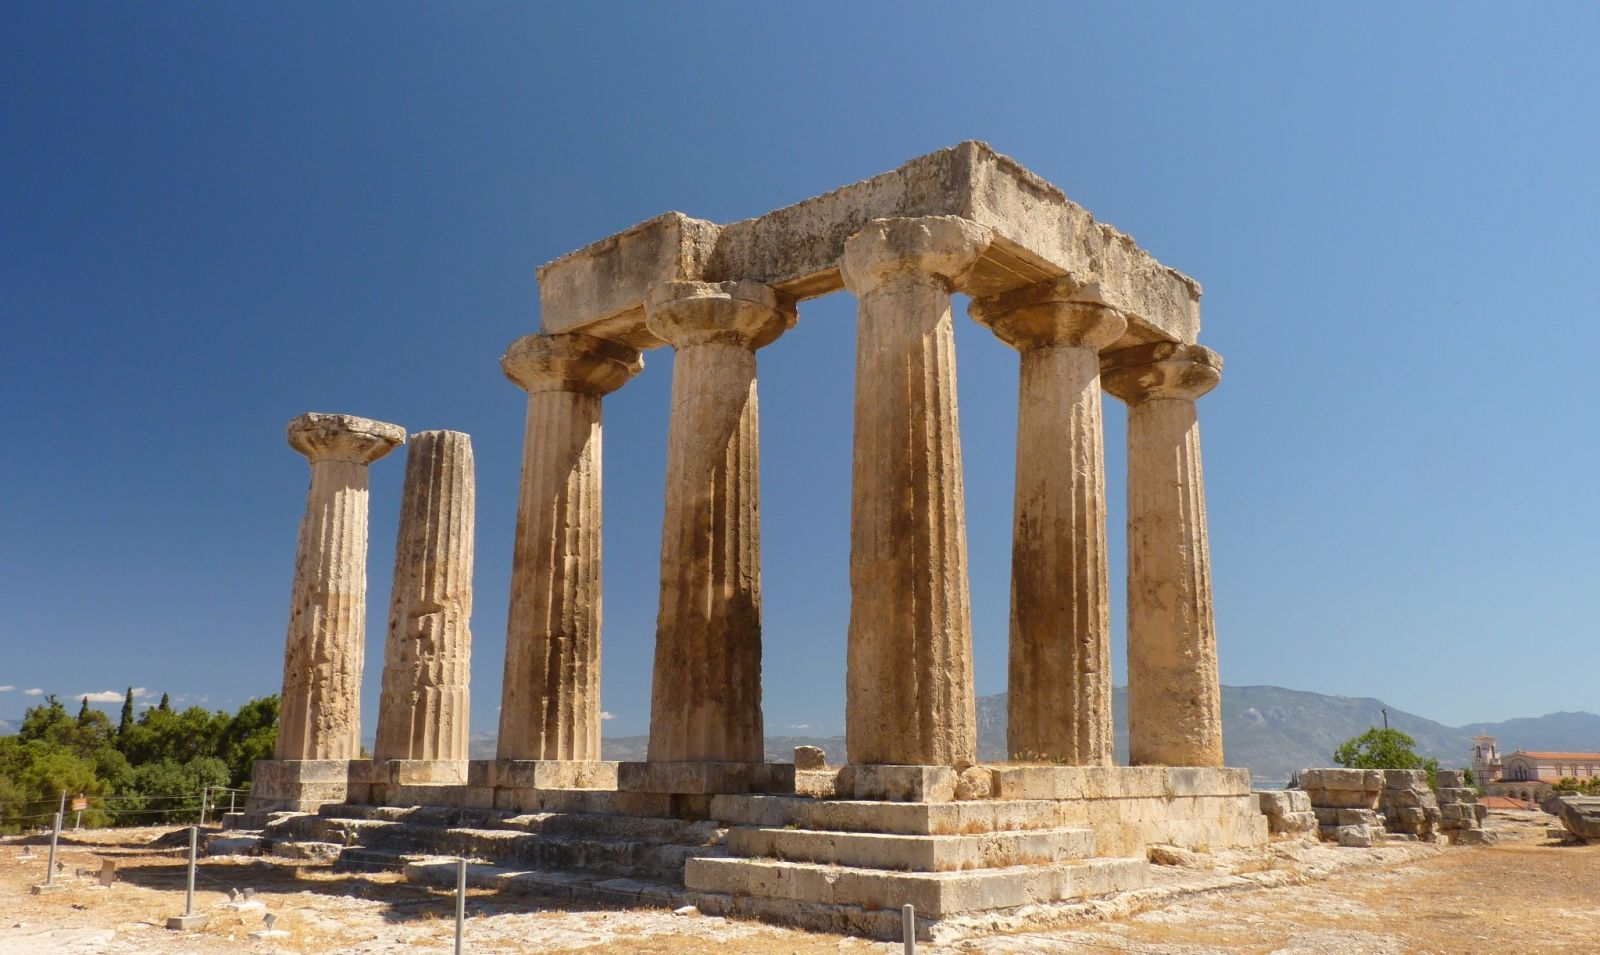
\includegraphics[width=0.6\textwidth]{exam-cover-06}

  \vspace{5mm}

  \textbf{\Huge{Level Three Calculus}}

  \vspace{2mm}

  \textbf{\Huge{Integration}}
\end{center}

\vspace{5mm}

\noindent
\large{There are three questions, worth a total of \numpoints\ marks.\\
       Attempt ALL questions, showing all working.\\
       Read questions carefully before attempting them.\\
       Marks are available for partial answers.\\
       The amount of time expected to be spent per question may not necessarily correlate ``nicely'' to the number of marks.\\
       Diagrams may be used to support answers.\\
       Candidates who do not provide diagrams for some questions may be disadvantaged.\\
       Some marks are given for clarity and neatness of solutions or proofs.}
\vspace{2mm}

\begin{tabular}{ll}
  \textbf{Time Allowed:}& One Hour\\
  \textbf{Achieved:}& 9 marks\\
  \textbf{Merit:}& 15 marks\\
  \textbf{Excellence:}& 21 marks
\end{tabular}

\vfill

\begin{center}
  \gradetable[h][questions]
  \vspace{2mm}

  \textbf{Available Grades:} \textit{Not Achieved}\quad\textit{Achieved}\quad\textit{Merit}\quad\textit{Excellence}
\end{center}

\end{coverpages}

\begin{questions}
  \question
    \begin{parts}
      \part For i. and ii., find the indefinite integrals. \textbf{Do not forget the constant of integration.}
        \begin{subparts}
          \subpart[1]
            \begin{displaymath}
              \rint \frac{1}{\sqrt{2x + 2}} \dif{x}
            \end{displaymath}
          \subpart[1]
            \begin{displaymath}
              \rint \sec^2 (x) \sec(\tan (x)) \tan(\tan(x)) \dif{x}
            \end{displaymath}
        \end{subparts}
      \part[3] Find the area of the region bounded by $ y = 1/x $, $ y = 1/x^2 $, and $ x = 2 $.
      \part[3] Find the general solution to the differential equation $ \od{y}{x} = \tan y \tan x $.
    \end{parts}
  \question
    \begin{parts}
      \part[3] Consider the following integral.
            \begin{displaymath}
              \pi \rint^{5}_1 (x^2 e^{-x})^2 \dif{x}.
            \end{displaymath}
            Complete the following table, and use Simpson's rule with an interval length of 0.5 to approximate the value
            of the definite integral.
            \begin{center}
              \def\arraystretch{1.5}%  1 is the default, change whatever you need
              \begin{tabular}{|c|c|}          \hline
                $ x $ & \mathstrut$ (x^2 e^{-x})^2 $\\\hhline{|=|=|}
                1.0   &                   \\\hline
                1.5   & 0.2520            \\\hline
                2.0   &                   \\\hline
                2.5   & 0.2632            \\\hline
                3.0   &                   \\\hline
                3.5   & 0.1368            \\\hline
                4.0   & 0.0859            \\\hline
                4.5   & 0.0506            \\\hline
                5.0   & 0.0284            \\\hline
              \end{tabular}
            \end{center}
        \part[2] Find $ k $ such that $\rint^k_1 \frac{\ln x}{x} \dif{x} = 5 $.
        \part[3] The Bank of Money (figure \ref{fig:bank}) advertises that a particular savings account package has continuously compounding
              interest at a rate of 4\% per annum. Express this as a differential equation, and hence find the accumulated interest on an
              initial deposit of \$2500 after four years.
            \begin{figure}
              \centering
              
\includegraphics[width=0.4\textwidth]{bank}
              \caption{A bank.\label{fig:bank}}
            \end{figure}
    \end{parts}

  \clearpage
  \question
    \begin{parts}
      \part[3] The average value of a function $ f $ on the interval $ a \leq x \leq b $ is defined to be
            \begin{displaymath}
              f_\text{avg} = \frac{\rint^b_a f(x) \dif{x}}{b - a}.
            \end{displaymath}
            The temperature $ T $ (in \si{\celsius}) of Napier $ t $ hours after 9 am on a particular day was modelled by
            \begin{displaymath}
              T(t) = 20 + 8\sin \left(\frac{\pi t}{12} \right).
            \end{displaymath}
            Find the average temperature during the period from 9 am to 9 pm.
      \part[2] The height of an obelisk, like that pictured in figure \ref{fig:obelisk}, is \SI{18}{\metre}. A horizontal
            cross-section at a distance $ x $ metres from the bottom is a rectancle of side lengths $ (3 - 0.1x) $ and $ (4 - 0.2x) $.
            Use integration to find the volume of the obelisk.
            \begin{figure}
              \centering
              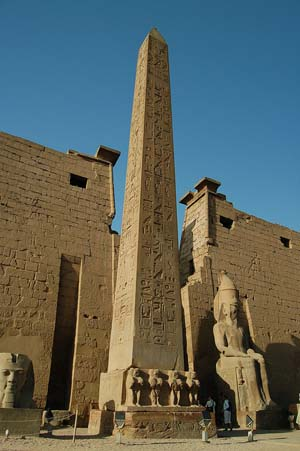
\includegraphics[height=0.2\textheight]{obelisk}
              \caption{An Egyptian obelisk.\label{fig:obelisk}}
            \end{figure}
      \part[3] Suppose that
            \begin{displaymath}
              1 = \rint^{2m}_m x \cos(mx^2) \dif{x}.
            \end{displaymath}
            Show that
            \begin{displaymath}
              m = \cos \frac{5m^3}{2} \sin \frac{3m^3}{2},
            \end{displaymath}
            and conclude that $ m \leq 1 $.
    \end{parts}
\end{questions}
\end{document}
